\documentclass[../main]{subfiles}
\begin{document}
\centering
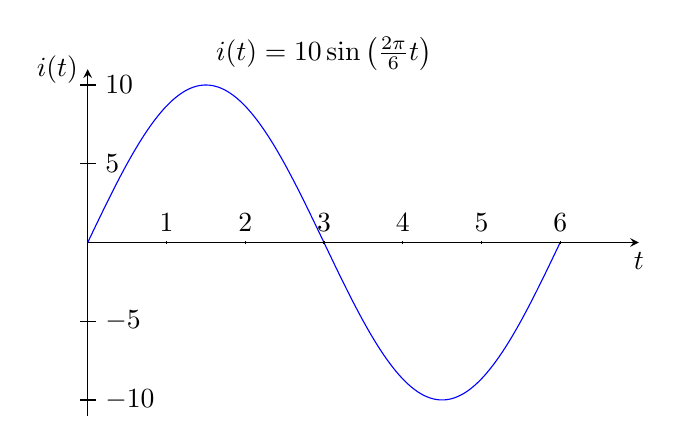
\begin{tikzpicture}[xscale=1,yscale=0.2]
  \draw[-stealth] (0,0) -- (7,0) node [below]{$t$};
  \draw[-stealth] (0,-11) -- (0,11) node [left]{$i(t)$};
  \draw[domain=0:6,samples=200,blue] plot (\x,{10*sin((2*pi/6)*\x r)});
  \foreach \x in {1,2,3,4,5,6}
    \draw (\x,-0.1) -- (\x,0.1) node [above] {$\x$};
  \foreach \y in {-10,-5,5,10}
    \draw (-0.1,\y) -- (0.1,\y) node [right] {$\y$};
  \node at (3,12) {$i(t)=10\sin\left(\frac{2\pi}{6}t\right)$};
\end{tikzpicture}






\end{document}
